\documentclass[11pt,a4paper]{article}

\usepackage{hyperref}
\usepackage{graphicx}
\usepackage{amssymb}
\usepackage{amsmath}
\usepackage{amsthm}
\usepackage[margin=19mm]{geometry}
\usepackage{natbib}
\usepackage{bm}
\usepackage[toc,page]{appendix}
\usepackage{booktabs}
\usepackage{listings}
%\usepackage{url}
%\usepackage{fancyhdr}
\usepackage{fancyvrb}
\usepackage{lscape}
%\usepackage{pdfsync}
\usepackage{rotating}
\usepackage{multirow}
\usepackage[nodisplayskipstretch]{setspace} \setstretch{1.5}
\let\oldv\verbatim
\def\verbatim{\par\setstretch{0.9}\oldv}
\usepackage[table]{xcolor}
\usepackage{algorithm,algorithmic}

%\renewcommand{\headrulewidth}{0.5pt} %Do not print a rule below the header
%\renewcommand{\footrulewidth}{0pt} %Do not print a rule above the footer

\bibpunct{(}{)}{;}{a}{,}{,}

%\renewenvironment{tabbing}{\linebreak \texttt \sl}{\linebreak}
\newcommand{\mP}{\mathbf{P}}
\newcommand{\I}{\mathbf{I}}
\newcommand{\K}{\mathbf{K}}
\newcommand{\Z}{\mathbf{Z}}
\newcommand{\X}{\mathbf{X}}
\newcommand{\Q}{\mathbf{Q}}
\newcommand{\A}{\mathbf{A}}
\newcommand{\C}{\mathbf{C}}
\newcommand{\mL}{\mathbf{L}}

\newcommand{\undertilde}[1]{\underset{\widetilde{}}{#1}}
\newcommand{\threeScript}[3]{
	\!\begin{smarray}{l}
  		{#1}\\ \hlx{s[-5pt]}
  		{#2}\\ \hlx{s[-5pt]}
  		{#3}
 	 \end{smarray}
}
\renewcommand{\baselinestretch}{1.5}
\setlength{\abovecaptionskip}{5pt}
\setlength{\belowcaptionskip}{-1pt}

\newtheorem{mydef}{Definition}

\floatname{algorithm}{Pseudocode}

\newcommand{\disfrac}{\displaystyle \frac}

\hypersetup{
    bookmarks=true,         % show bookmarks bar?
    unicode=false,          % non-Latin characters in Acrobat’s bookmarks
    pdftoolbar=true,        % show Acrobat’s toolbar?
    pdfmenubar=true,        % show Acrobat’s menu?
    pdffitwindow=false,     % window fit to page when opened
    pdfstartview={FitH},    % fits the width of the page to the window
    pdftitle={My title},    % title
    pdfauthor={Author},     % author
    pdfsubject={Subject},   % subject of the document
    pdfcreator={Creator},   % creator of the document
    pdfproducer={Producer}, % producer of the document
    pdfkeywords={keyword1} {key2} {key3}, % list of keywords
    pdfnewwindow=true,      % links in new window
    linktoc = page,
    colorlinks=true,       % false: boxed links; true: colored links
    linkcolor=blue,          % color of internal links
    citecolor=blue,        % color of links to bibliography
    filecolor=magenta,      % color of file links
    urlcolor=cyan           % color of external links
}

%###################################################################################################
%Writing starts here!!
%
%###################################################################################################

\begin{document}
\title{Introduction}
\author{Kevin Chang}
\date{\today}
\maketitle

%\tableofcontents
%\chapter{Introduction}\label{chap:intro}

\section{Introduction}
All studies require that researchers conduct one or more experiments to make confident claims to support or refute a particular hypothesis. A carefully thought out plan for an experiment is essential, and is an important discipline of study called \emph{experimental design}. The initial foundations of statistical approach to design the experiments were laid by \cite{Fisher1935} in the field of agriculture, but it is now applicable to almost all sciences. \citeauthor{Fisher1935}'s main focuses were in the principles of comparison, randomisation, replication, blocking, orthogonality and the use of factorial treatments in connection with the design of experiment. These concepts should be implemented in a carefully thought out experiment if the researcher wishes the result to stand up to scrutiny.

Carefully thought out experimental design offers several advantages. First, the experiments are used to provide scientific evidences, so the researchers should design and conduct their experiment in such a way that there is reasonable confidence that the conclusion which are drawn from it reflect the truth, i.e.\
the experimental conclusion must be \emph{valid} \citep{Maxwell2004}. Second, the information obtained should increase per experiment versus an ad hoc approach, because a such experiment should protect the inability to distinguish the effects of interest from the nuisance sources of variation, i.e.\ \emph{confounding}. Further, the experimental design should provide an organised approach to conduct the experiment, to analyse the datasets and to interpret the results. Thus, the findings from the experiment should be reproducible, which facilitates the communication between statisticians and researchers \citep{Doyle2009}. 

This thesis focuses on the \emph{quantitative high-throughput biotechnologies experiment}. This type of experiment involves the measurement of intracellular molecular species, such as genes, proteins or metabolites, of interest in terms of linking changes in their abundances to the presence or severity of conditions of interest. However, their in-vivo measurement is generally not possible without the use of high-throughput biotechnologies which simultaneous testing on an sample comprises large numbers of candidate molecular species \citep{Janzen2002}. An example can be \emph{proteomics experiment} which is the identification and quantification of the entire complement of proteins at a given condition within a cell for a single sample. The measurement of the protein abundances is achieved by the Multi-dimensional Protein Identification Technology (MudPIT). 

Proteomics experiments generally have a \emph{two-phase} structure. The organisms are first perturbed by the experimental conditions of interest, i.e.\ the \emph{Phase~1 experiment}. Since protein abundance cannot be measured directly from the organisms, the organ must be harvested and the proteins are extracted for the subsequent laboratory based experiment, i.e. the \emph{Phase~2 experiment}, which uses MudPIT to measure proteins' abundances. Thus, such experiments are also known as \emph{two-phase experiments}. 

Due to the high variation between different MudPIT experiments, a \emph{multiplexing} technology is introduced that allows the simultaneous analysis of multiple samples, for example isobaric Tags for Relative and Absolute Quantitation (iTRAQ$^{\textrm TM}$) \citep{Ross2004}. Another advantage of multiplexing is that it reduces overall experimental costs. However, complications arise in the design of the Phase~2 experiment, specifically in how the samples should be measured using this multiplexing technology. 

This chapter establishes some general insights into the two-phase experiments. Sections~\ref{sec:introTwoPhase} to \ref{sec:brien2011} describes the evolution of the methods surrounding the two-phase experiments over recent decades. Moreover, Section~\ref{sec:proteomicExpt} details the biological background of the MudPIT-iTRAQ$^{\textrm TM}$ experiments. Section~\ref{sec:oberg} describes some recent works in the experimental design for the proteomics experiments. Finally, Section~\ref{sec:overview} presents a brief overview of this thesis.

\section{The introduction of two-phase experiments by McIntyre}
\label{sec:introTwoPhase}
The concepts of two-phase experiments were first introduced by \cite{McIntyre1955}, who investigated the effects of four light treatments on the synthesis of tobacco mosaic virus in tobacco leaves. The Phase~1 experiment comprised two $4 \times 4$ arrays consisting of four leaves taken from each of eight infected plants by the virus. The four light treatments were then assigned to the plants and leaves such that each treatment occurs only once within each row and column in each of two $4 \times 4$ square arrays. This assignment is also known as \emph{Latin square design} \citep{Bailey2008}. The Phase~1 experiment thus yielded 32 observations. However, the virus content of each leaf could not be measured directly from the test plants used in the Phase~1 experiment. Therefore, in the Phase~2 experiment, the virus content of each leaf was assayed by expressing sap and inoculated using the half leaves of assay plant, where the countable lessons are appeared. 

The Phase~2 experiment comprised four $4 \times 4$ arrays consisting of four leaves taken from each of 16 assay plants. Since each leaf was further divided into two halves, the Phase~2 design can take the form of two sets of Latin square designs superimposed on each other, an arrangement also known as the \emph{Greaco-Latin square design}. Hence, a total of 128 samples are measured in the Phase~2 experiment. Given that the Phase~1 experiment involved 32 samples, each sample was replicated four times in the Phase~2 experiment. This experiment provides a good example of a two-phase experiment that requires two different experimental designs, where the first design prepares a set of test plants that were perturbed by the light treatments of interest while the second design allows the measurements of the lesions on the assay plants that correspond to the virus content of a certain treatment and test plant from the Phase~1 experiment. 

If multiple measurements on each sample from the Phase~1 experiment are not made in the Phase~2 experiment, the variance of treatment differences will comprise both biological and technical variation, i.e.\ the variation between the test plants will be confounded with the measurement error. These multiple measurements are also known as \emph{technical replicates}, i.e.\ measuring the multiple subsamples from each Phase~1 biological sample. \cite{McIntyre1955} stated that this replication is only required if the Phase~2 experiment introduces large and uncontrollable variation. For the light treatment example mentioned above, each treatment is replicated four times in Phase~1. Additionally, each sample in the Phase~1 experiment is measured four times in the Phase~2 experiment. Thus, both types of replication are used in the light treatment experiment. 

The construction of the ANOVA table with EMS is shown to usefully illustrate the linear combination of the variance components because it shows the estimation of the error variance for the treatment effects. \cite{McIntyre1955} discussed three further observations using these error variances and based on the light treatment experiment. First, he demonstrated that if the Phase~1 design remains unchanged while the Phase~2 design is modified, the error variances for the treatment comparisons are different with different Phase~2 design. This is because the different designs cause different combinations of the variance components. Second, if the design is modified to have more technical replicates, the error variance for the treatment effects can be reduced, but the time required to complete the experiment is increased. Third, if the design is modified to eliminate biological replication, the error variance for the treatment effects increases. This is because the error variance includes the variation among leaves from single plants from both the Phase~1 and 2 experiments. 

\section{New ANOVA by \cite{Curnow1959}}
\cite{Curnow1959} revisited \citeauthor{McIntyre1955}'s light treatment experiment and generated a new ANOVA table. The new ANOVA table is better than that presented by \cite{McIntyre1955}, because it shows the decomposition of the total sum of squares (SS) into each source of variation associated with each treatment or block factor. Table~\ref{tab:Curnow1959}, which includes only the treatment and residual SS, shows that the treatment effects can be estimates in both ``Between and Within Leaves Within Assay Plants''. The components in EMS are $\sigma_{\epsilon}^2$ which denotes the variation between halves within leaves of assay plants, $\sigma_{\Delta}$ which denotes the variation between leaves in assay plants, $\sigma_{L}$ which denotes the variation between leaves in test plants and $\theta$ which is the differences between the light treatments. The first estimate of the treatment effects contains $\sigma_{\Delta}^2$, whereas the second estimate does not. \cite{Curnow1959} labels these first and second estimations of the treatment effects as the \emph{sums} and \emph{differences} analyses, respectively, which are equivalent to \emph{inter} and \emph{intra}-block analyses, respectively. \cite{Curnow1959} then showed how to combine the inter- and intra-block analyses using the weights computed from the error variance of treatment comparison. 
 
\begin{table}[ht]
\centering
\caption{Partial theoretical ANOVA table by \cite{Curnow1959}.}
\begin{tabular}{lrl} 
\toprule 
\multicolumn{1}{l}{\textbf{Source of Variation}} & \multicolumn{1}{l}{\textbf{DF}} & \multicolumn{1}{l}{\textbf{EMS}}\\ 
\midrule 
Between Leaves in Assay Plants & & \\ 
\quad Treatment & $3$ & $\sigma_{\epsilon}^2 + 2\sigma_{\Delta}^2 + 2\sigma_{L}^2 + 16\theta$ \\ 
\quad Residual & $15$ & $\sigma_{\epsilon}^2 + 2\sigma_{\Delta}^2 + 2\sigma_{L}^2$ \\  \hline
Within Leaves in Assay Plants & & \\
\quad Treatment & $3$ & $\sigma_{\epsilon}^2 +  2\sigma_{L}^2 + 16\theta$ \\ 
\quad Residual & $15$ & $\sigma_{\epsilon}^2 +  2\sigma_{L}^2 $ \\  
\bottomrule 
\end{tabular}
\label{tab:Curnow1959} 
\end{table} 
 
In contrast with the \cite{McIntyre1955}, who performed the unweighted pooled estimation of treatment effects in the ``Between and Within Leaves Within Assay Plants''; thus the estimation of treatment effects is combined and showed in the ANOVA table in Table~\ref{tab:McIntyre1955}. Furthermore, the total degrees of freedom (DF) of the light treatment experiment is 127, but the total DF from the ANOVA table by \cite{McIntyre1955} is 155, which is incorrect. Additionally, \cite{McIntyre1955} also omitted the 3 DF for the Greaco-Latin Squares in the original ANOVA table. Therefore, the new ANOVA table by \cite{Curnow1959} took account of all 127 DF from the light treatment experiment, and thus provides a first step towards developing a better analytical procedure for the two-phase experiments. 
 
\begin{table}[ht]
\centering
\caption{Partial theoretical ANOVA table by \cite{McIntyre1955}.}
\begin{tabular}{lrl} 
\toprule 
\multicolumn{1}{l}{\textbf{Source of Variation}} & \multicolumn{1}{l}{\textbf{DF}} & \multicolumn{1}{l}{\textbf{EMS}}\\ 
\midrule 
Treatment & $3$ & $\sigma_{\epsilon}^2 + \sigma_{\Delta}^2 + 4\sigma_{L}^2 + 32\theta$ \\ 
Residual & $15$ & $\sigma_{\epsilon}^2 + \sigma_{\Delta}^2 + 4\sigma_{L}^2$ \\  
\bottomrule 
\end{tabular}
\label{tab:McIntyre1955} 
\end{table} 

\section{Non-orthogonal structure in the two-phase experiment}
\cite{Wood1988} discussed the non-orthogonal block structure of the two-phase experiments, which occurs when the block factor from the Phase~1 experiment is confounded with multiple block factors in the Phase~2 experiment. The orthogonality can be measured by the \emph{efficiency factor} which is the proportion of treatment information presented for the intra-block analysis \citep{Yates1936}. The efficiency factor thus should also be used to measure the proportion of the block information for cases involving non-orthogonal structure as shown by \citep{Wood1988}. 

This thesis studies the cases of block or treatment factor in the Phase 1 experiment is confounded with multiple block factors in the Phase~2 experiment, which can occur in two different ways. The first is that the DF of block effects from the Phase~1 experiment are split into inter- and intra-blocks. This can be shown in the ANOVA table given by \cite{Curnow1959} where the 6 DF associated with the leaf positions of the test plants are split into two SS, both estimated with 3 DF. The first SS is confounded with the whole leaves of the assay plants while the second is orthogonal to them. The efficiency factor for both SS can be shown to be 1. The second origin is that the DF of block effects from the Phase~1 experiment remain intact. Table~\ref{tab:Wood1988}, is the artificial design presented by \cite{Wood1988}, shows the allocation of the Phase 1 units to the Phase 2 blocks. In the ANOVA, all three DF associated with the units SS of the Phase~1 experiment are estimated in both the Between and Within Blocks. The separation for this case is then measured using the efficiency factor. Both types of confounding should be minimised, because they can increase the error variance of the treatment effects and affect on how the test for the treatment effects in performed. Chapters 3 and 4 describe the methods used to find the optimal design and also remain aware of the issues in the non-orthogonal structures and how they affect the ANOVA. 

\begin{table}[ht]
\centering
\caption{Phase~2 design showing the allocation of Phase~1 units to Phase~2 blocks in the artificial design by \cite{Wood1988}.}
\begin{tabular}{ccccc} 
\bf Block & 1 & 2 & 3 & 4 \\ \hline
& 1 & 2 & 3 & 4 \\  
& 1 & 2 & 3 & 4 \\  
& 2 & 3 & 4 & 1 \\   \hline
\end{tabular} 
\label{tab:Wood1988}
\end{table}

\section{Constructing the analysis of variance table}
\label{sec:Brien1983}
Neither \cite{McIntyre1955} nor \cite{Curnow1959} described how their ANOVA tables were determined. \cite{Brien1983} thus presented a generalised procedure for determining the ANOVA table for both single- and two-phase experiments. Notably, the presented ANOVA consists only the decomposition of the total DF into each source of variation, without the EMS. This section briefly describes the procedure presented by \cite{Brien1983} and simultaneously introduces some basic terminologies used in experimental design.

Before constructing the ANOVA table, the overall structure of the experiment must be determined. The first step is to identify the treatment and block factors in the experiment and the observational unit. The observational unit is the smallest measure quantity of experimental material \cite{Bailey2008}. The second step is to divide the factors into different sets sharing the same randomisation scheme, which \cite{Brien1983} called \emph{tiers}. \emph{Randomisation}, one of the important principles in the experimental design presented by \cite{Fisher1935}, involves the assignment of one set of objects to another. The main purpose of randomisation is to enable researchers to obtain a data set with minimal systematic bias. 

A single-phase experiment, in general, has two tiers of factor. The first tier consists of the factors that jointly identify the observational unit in the absence of randomisation. \cite{Nelder1965A} also referred to first tier factors as \emph{block} factors. The second tier factors are those level combinations that are directly associated with the factors at the first tier based on the randomisation. The second tier factors thus are what \cite{Nelder1965B} termed \emph{treatment} factors. The smallest unit in the first tier to which the treatment can be assigned is also known as the \emph{experimental unit}. The last step is to determine the relationships between the factors within each tier. \cite{Wilkinson1973} developed a symbolic syntax which to represent the relationship between the block and treatment factors, namely block and treatment structures, respectively. \cite{Brien1999} termed this representation a \emph{structure formula}. \citeauthor{Wilkinson1973}'s syntax was originally developed to generate and analyse the ANOVA models in the GenStat statistical analysis program, but is now widely used in many statistical packages. Two basic operations described by \cite{Wilkinson1973} are used to represent block and treatment structures, namely \emph{crossing} denoted by an asterisk, $*$, and \emph{nesting}, denoted by a slash, $/$. 

A two-phase experiment, in general, involves three tiers of factors, two of block factors and one of treatment factors. Consequently, two-phase experiments are also known as \emph{multi-tiered experiments}. Tiers 1 and 2 comprise block factors from the Phase~2 and 1 experiments, respectively. Tier 3 contains the treatment factors of the two-phase experiments. 

The ANOVA table can be obtained once the structure formula for every tier of the experiment is determined. The first step is to expand the structure formulae for each tier, which yields a set of terms based on the rules described by \cite{Wilkinson1973}. The terms from the first tier form an initial structure of the ANOVA table. Meanwhile, the terms from the second tier are included in the table under the terms of the first tier with indentation, and only if the two terms from different tiers are confounded. The confounding between the terms can be examined using the contrasts generated from each term. The two-phase experiment includes an additional tier. Therefore, the terms from tier 3 are grouped with those from tiers 1 or 2, with another indentation in the event of confounding between terms from the two different tiers. 

Using the example of wine-evaluation experiment described by \cite{Brien1983}, the factors of the field experiment are Blocks, Plots and Treatments with $b$, $p$ and $p$ levels, respectively. The factors of the tasting experiment are Tasters and Sittings with $t$ and $bp$ levels, respectively. The observational unit is the wine given to a taster at a particular sitting. The level combination of Taster and Sitting factors cannot be randomised; thus, Taster and Sitting factors formed the first tier. The levels of Block and Plot factors combination are randomised to Sittings within each Taster; thus, the Block and Plot factors formed the second tier. Finally, the levels of Treatment are randomised to the Plots within each Block; thus, the Treatment factor forms the third tier. The structure formulae of Phase~2 and 1 block tiers can be written as
\begin{eqnarray}
\label{eq:stru1}&&\mathrm{Taster/Sitting},\\
\label{eq:stru2}&&\mathrm{Block/Plot}
\end{eqnarray}
and the treatment tier is expressed as
\begin{equation}\label{eq:stru3}
\mathrm{Treatment.}
\end{equation}
The structure formulae in (\ref{eq:stru1}) and (\ref{eq:stru2}) can then be expanded to 
\begin{equation}\label{eq:stru1expanded}
\mathrm{Taster + Taster.Sitting}
\end{equation}
and 
\begin{equation}\label{eq:stru2expanded}
\mathrm{Block + Block.Plot},
\end{equation}
respectively, where $\mathrm{Taster.Sitting}$ and $\mathrm{Block.Plot}$ denote ``Between Sittings Within Tasters'' and ``Between Plots Within Blocks'', respectively. After studying the relationship between the terms from different tiers, the ANOVA table, with only the decomposition of the DF, can be derived and is given in Table~\ref{tab:Brien1983}. The indention on the line with Treatment indicate that the effects of Treatments are confounded with $\mathrm{Block.Plot}$. For a more detailed description of these procedures see \cite{Brien1983}.

\begin{table}[ht]
\centering
\caption{ANOVA table of the wine-evaluation experiment described by \cite{Brien1983}.}
\begin{tabular}{lrl} 
\toprule 
\multicolumn{1}{l}{\textbf{Source of Variation}} & \multicolumn{1}{l}{\textbf{DF}} \\ 
\midrule 
Between Tasters & $t-1$  \\ 
Between Sittings Within Tasters & $t(bp-1)$ \\  
\quad Between Blocks  & $b-1$  \\ 
\quad Between Plots Within Blocks & $b(p-1)$ \\ 
\quad \quad Treatment & $p-1$  \\ 
\quad \quad Residual & $(b-1)(p-1)$ \\ 
\quad Residual & $(bp-1)(t-1)$ \\ 
\bottomrule 
\end{tabular}
\label{tab:Brien1983} 
\end{table} 

\cite{Brien1983} concluded by expressing that the randomisation between the factors of different tiers can alter the relationships among factors within each tier. Consider, for instance, an experiment arranged in a Row-Column design; the relationship between the Row and Column factors is \emph{crossed}. Consider the Plots as the observational units for this experiment, then suppose a randomised block design is to be superimposed on the Plots, with Treatment being randomised to the Plots within each Row. The effects of Treatment then becomes confounded with the Column factor and the relationship between the Row and Column factors becomes \emph{nested}. Therefore, the experimental structure depends on both the innate physical structure of the experimental material and on how the randomisation is employed. 

\section{Complex two-phase experiments}\label{sec:Brien1999}
A complex two-phase experiment has at least one term in the structure formula of the third tier that is non-orthogonal to the multiple terms in the structure formula of the second tier, which themselves are non-orthogonal to multiple terms in the structure formula of the first tier. Thus, there are two sets of efficiency factors, denoted by $E$, to describe the non-orthogonal relationship between the terms of different tiers, as mentioned by \cite{Wood1988}. 

The procedures described in \cite{Brien1983} to construct the ANOVA table only provide the decomposition of the total DF. \cite{Brien1999} thus described an algorithm using two types of \emph{sweeping} operations to construct the ANOVA table which provides the estimation of the effects for each source of variation for any single- or two-phase experiment. 

The sweeping operations were introduced by \cite{Wilkinson1970} and \cite{Payne1977}. Every experiment generates $n$ responses which can be viewed as a data vector, commonly denoted by $\bm{y}$, with length $n$ in the $n$-dimensional space \citep{Payne1977}. The standard sweeping operation estimates the effects of a term from the expanded structure formula and then subtracts the estimated effects from the current working vector which is then become the working vector for the next sweep \citep{Brien1999}. 

The single-phase field experiment described in Section~\ref{sec:Brien1983} is used to demonstrate the sweeping operations. The factor of this experiment consists of Blocks, Plots and Treatments with $b$, $p$ and $p$ levels, respectively. The expanded structure formulae of the block and treatment tiers are given in (\ref{eq:stru2expanded}) and (\ref{eq:stru3}), respectively. For this experiment to be complex, the Treatment term in (\ref{eq:stru3}) has to be non-orthogonal to the $\mathrm{Block}$ and $\mathrm{Block.Plot}$ term in (\ref{eq:stru2expanded}). The grand mean of the dataset from any experiment can be estimated which automatically become part of structure formulae \citep{Payne1977}. Thus, the first sweep is for the grand mean, i.e.\ removing the effects of grand mean, using the \emph{reanalysis sweep}, which can be expressed by 
\begin{equation}
\mathbf{I} - E_{G} \mP_{G}
\end{equation}
where $\mathbf{I}$ is the $n \times n$ identity matrix, while $E_{G}$ and $\mP_{G}$ are the efficiency factor and projection matrix associated with the grand mean. The $\mP_{G}$ is defined as 
\[ {\K}({\K}'{\K})^{-1}{\K}'\]
where $\K$ denote $n \times n$ averaging matrix with all elements equal to ${n}^{-1}$. In general, the reanalysis sweep is to sweep the non-orthogonal terms from the data vector; the sweep to remove the effect of Block term from the data vector is given by  
\[\mathbf{I} - E_B \mathbf{P}_B,\]
where $E_{B}$ and $\mP_{B}$ are the efficiency factor and projection matrix associated with the Block term. The second type of sweep operator is the \emph{pivotal sweep} which is used to estimate the effects of the associated terms. Thus, the pivotal sweep for estimating the effect of Treatment term is given by  
\begin{equation}
E_T \mathbf{P}_T,
\end{equation}
where $E_{T}$ and $\mP_{T}$ are the efficiency factor and projection matrix associated with the Treatment term. This sweep is required for the terms of the structure formula for the first (block) tier before performing the same sweep for the terms in the structure formula for the second (treatment) tier that are confounded with it. Therefore, the sweeping sequence to estimate the effects of Treatment in Between Blocks for the field experiment is given by 
\[E_T \mP_T E_B \mP_B (\I - E_K \mP_G)\bm{y},\] 
which consists of two pivotal sweeps for the Treatment and Block terms, because the effects of Treatment are confounded with the Between Blocks, and a reanalysis sweep for the grand mean. The sweeping sequence for the estimation on the other effects of the experiment can also be derived from a combination of the reanalysis and pivotal sweeps. Thus, the ANOVA table can be constructed with the effects for each source of variation. 

\cite{Brien1999} extended the sweep algorithm for the two-phase experiment by performing additional sweeps for terms from the structure formula of third tier. Using the example of the two-phase wine-evaluation experiment described in Section~\ref{sec:Brien1983}, the effects of Treatment in Between Plots Within Blocks and Between Sittings Within Tasters are given by 
\[\mP_T \mP_P (\I - \mP_B) \mP_S (\I - \mP_J) (\I - \mP_G)\bm{y}, \]
where $mP_P$, $mP_S$ and $mP_J$ denote the projection matrix associated with Plots, Sittings and Tasters, respectively. Since all block and treatment information is intact, all the efficiency factors are unity and are not written in the expression. 

To summarise, \cite{Brien1999} demonstrated the use of the reanalysis and pivotal sweep operators to construct the ANOVA table. Chapter 2 further discusses these method in the constructing the ANOVA table.

\section{Works by Brien and Bailey} 
\cite{Brien2006b} described how randomisation can be achieved for the multi-tiered experiment, which involves at least three tiers of factors. Thus, the multi-tiered experiment also covers the two-phase experiment. As \cite{Brien1983} pointed out, randomisation can affect the structure of the experiments. For an experiment that involves with three tiers of factors, a randomisation typically must be perform twice: (1) for the allocation of treatments to experimental units in the Phase~1 experiment, and (2) for the allocation of experimental units from the Phase~1 experiment to the experimental units in the Phase~2 experiment. The randomisation procedure for the multi-tiered experiment thus is termed \emph{multiple randomisation} \citep{Brien2006b}.  

\cite{Brien2006b} then compared and contrasted six types of multiple randomisation with three tiers of experiments, namely composed, coincident, independent, double, randomised-inclusive and non-randomised-inclusive multiple randomisations. These six multiple randomisations differ in both the direction and interaction of the factors between different tiers. For a more detailed description of these multiple randomisations see \cite{Brien2006b}.

\cite{Brien2009, Brien2010} also published two papers on the aspects of orthogonal decomposition of the data space for the multi-tiered experiments with respect to different types of multiple randomisation.

The example of single-phase field experiment described in Section~\ref{sec:Brien1983} is used to demonstrate the orthogonal decomposition method discussed by \cite{Brien2009, Brien2010}. The $\mathrm{Treatment}$ term in (\ref{eq:stru3}) is again assumed to be non-orthogonal to both the $\mathrm{Block}$ and $\mathrm{Block.Plot}$ terms in (\ref{eq:stru2expanded}). The two sets of matrices, containing the orthogonal projectors which correspond to the terms in the expanded structure formulae, of first (block) and second (treatment) tiers are denoted by $\mathcal{Q}_1$ and $\mathcal{Q}_2$, respectively. Each orthogonal projector in $\mathcal{Q}_1$ of the field experiment can be expressed as
\begin{equation}\label{eq:orthField}
\{\Q_{G}, \Q_{B}, \Q_{P(B)}\}
\end{equation}
where each orthogonal projector can be computed from the projection matrix defined in Section~\ref{sec:Brien1999}, i.e.\
$\Q_{G} = \mP_G$, $\Q_{B} = \mP_{B}(\I - \mP_G) =  \mP_{B} - \mP_G$ and $\Q_{P(B)} = (\I - \mP_{B})(\I - \mP_G) = \I  - \mP_{B}$. Each of these orthogonal projectors in $\mathcal{Q}_1$ also corresponds to a \emph{stratum} in the ANOVA table of the experiment. The orthogonal projector in $\mathcal{Q}_2$ is then
\begin{equation}\label{eq:orthTrt}
\{\Q_{G}, \Q_{T}\}
\end{equation}
where
$\Q_{T} = \mP_{T}(\I - \mP_G) = \mP_{T}- \mP_G$.
The matrix set $\mathcal{Q}_1$ decomposed by the matrix set $\mathcal{Q}_2$ is expressed by
\begin{equation}\label{eq:decomp}
\mathcal{Q}_1 \rhd \mathcal{Q}_2
\end{equation}
which is 
\begin{equation}\label{eq:decompTerm}
 \{\Q_{G}, \Q_{B}  \rhd \Q_{T}, \Q_{B} \vdash \mathcal{Q}_2, \Q_{P(B)} \rhd \Q_{T}, \Q_{P(B)} \vdash \mathcal{Q}_2\}
\end{equation}
where $\Q_{B}  \rhd \Q_{T}$ and  $\Q_{P(B)} \rhd \Q_{T}$ denote the orthogonal projectors for the Treatment effects in the ``Between and Within Blocks strata'', respectively, while $\Q_{B} \vdash \mathcal{Q}_2$ and $\Q_{P(B)} \vdash \mathcal{Q}_2$ are the residual effects in the ``Between and Within Blocks strata'', respectively. Each element in (\ref{eq:decompTerm}) corresponds to the orthogonal projector of each line in the ANOVA table. The term $\Q_{B}  \rhd \Q_{T}$, in (\ref{eq:decompTerm}), denotes the Block decomposed by the effects of Treatment and is then defined as 
\[E_{TB}^{-1}\Q_{B}\Q_{T}\Q_{B} \]
where $E_{TB}$ denotes the efficiency factor of Block decomposed by the effects of Treatment. Another term $\Q_{B} \vdash \mathcal{Q}_2$, in (\ref{eq:decompTerm}), denotes the residual of $\mathcal{Q}_2$ in $\Q_{B}$ and is then defined as
\begin{equation}\label{eq:residual}
\Q_{B} \vdash \mathcal{Q}_2 = \Q_{B} - \sum_{\Q \in \mathcal{Q}_2} \Q_{B} \rhd \Q,
\end{equation}
where $\sum_{\Q \in \mathcal{Q}_2}$ denotes the summation over $\Q$ in $\mathcal{Q}_2$ with non-zero efficiency factors. Since the orthogonal projector for the grand mean, $Q_G$, is considered in $\mathcal{Q}_1$, the $$Q_G$$ can be ignored in $\mathcal{Q}_2$; thus, (\ref{eq:residual}) can be written as 
\[\Q_{B} - \Q_{B} \rhd \Q_{T}.\] 
Hence, each term in (\ref{eq:decompTerm}) can be re-written as 
\begin{equation}\label{eq:decompTermExpaned}
\{\Q_{G}, E_{TB}^{-1}\Q_{B}\Q_{T}\Q_{B}, \Q_{B} - \Q_{B}  \rhd \Q_{T}, E_{T P(B)}^{-1}\Q_{P(B)}\Q_{T}\Q_{P(B)}, \Q_{P(B)} -\Q_{P(B)} \rhd \Q_{T}\}
\end{equation}
where the two efficiency factors $E_{T B}$ and $E_{T P(B)}$ should sum to one. 

For the multi-tiered experiments, the decomposition method can be performed across the tiers. Using the example of the two-phase wine-evaluation experiment described in Section~\ref{sec:Brien1983}, three sets of orthogonal projectors derived from the structure formulae of each of the three tiers are denoted by $\mathcal{Q}_1$, $\mathcal{Q}_2$ and $\mathcal{Q}_3$, respectively. Each orthogonal projector in $\mathcal{Q}_1$ of the evaluation experiment can be expressed as  
\[\{\Q_{G}, \Q_{J}, \Q_{S(J)}\}, \]
where
$\Q_{J} =  \mP_{J} - \mP_G$ and $\Q_{S(J)} = \I  - \mP_{J}$.
The $\mathcal{Q}_2$ and $\mathcal{Q}_3$ consist of the orthogonal projector matrices of the field experiment, which are given previously in (\ref{eq:orthField}) and (\ref{eq:orthTrt}), respectively. The $\mathrm{Treatment}$ term in $\mathcal{Q}_3$ is assumed to be non-orthogonal to $\mathrm{Block.Plot}$ in $\mathcal{Q}_2$ for this case. The decomposition among the three tiers can be written as 
\[(\mathcal{Q}_1 \rhd \mathcal{Q}_2) \rhd \mathcal{Q}_3\]
which equals 
\begin{equation}\label{eq:decompTwoPhase}
\{\Q_{G}, \Q_{J}, \Q_{S(J)} \rhd \Q_B, (\Q_{S(J)} \rhd \Q_{P(B)}) \rhd \Q_{T}, (\Q_{S(J)} \rhd \Q_{P(B)}) \vdash \mathcal{Q}_3, \Q_{S(J)} \vdash \mathcal{Q}_2\},
\end{equation} 
where $(\Q_{S(J)} \rhd \Q_{P(B)}) \rhd \Q_{T}$ denotes the orthogonal projector for the Sittings Within Tasters decomposed by the Plots Within Blocks decomposed by the Treatments, which can be re-expressed to 
\[
E_{TP(B)}^{-1}E_{P(B)S(J)}^{-1} \Q_{T}\Q_{P(B)}\Q_{S(J)} \Q_{P(B)}\Q_{T},
\]
where $E_{TP(B)}$ and $E_{P(B)S(J)}$ are the efficiency factors used to adjust for the two decompositions. Another orthogonal projector $(\Q_{S(J)} \rhd \Q_{P(B)}) \vdash \mathcal{Q}_3$, in  (\ref{eq:decompTwoPhase}), denotes the residual in the Plots Within Blocks which decomposed in the Sittings Within Tasters. Since $\mathcal{Q}_3$ only contains $\Q_{T}$, orthogonal projector $(\Q_{S(J)} \rhd \Q_{P(B)}) \vdash \mathcal{Q}_3$ can be re-expressed to 
\[
E_{P(B)S(J)}^{-1}\Q_{P(B)}\Q_{S(J)} \Q_{P(B)} - \Q_{T}.
\]
Hence, (\ref{eq:decompTwoPhase}) can be re-written as 
\begin{eqnarray}
\nonumber &&\{\Q_{G}, \Q_{J}, E_{BS(J)}^{-1}\Q_B\Q_{S(J)}\Q_B,  E_{TP(B)}^{-1}E_{P(B)S(J)}^{-1} \Q_{T}\Q_{P(B)}\Q_{S(J)} \Q_{P(B)}\Q_{T},\\
\label{eq:decompTwoPhaseExpaned}&& E_{P(B)S(J}^{-1}\Q_{P(B)}\Q_{S(J)} \Q_{P(B)} - \Q_{T}, \Q_{S(J)} - \Q_B - \Q_{P(B)}\},
\end{eqnarray}
where each of these elements can be inserted into the ANOVA table as shown in Table~\ref{tab:Brien2010}.

\begin{table}[ht]
\centering
\caption{ANOVA table of the wine-evaluation experiment described by \cite{Brien1983}.}
\begin{tabular}{lrll} 
\toprule 
\multicolumn{1}{l}{\textbf{Source of Variation}} & \multicolumn{1}{l}{\textbf{DF}}  & \multicolumn{1}{l}{\textbf{Decomposition}}\\ 
\midrule 
Between Tasters & $t-1$  & $\Q_{J}$\\ 
Between Sittings Within Tasters & $t(bp-1)$ &\\  
\quad Between Blocks  & $b-1$  & $E_{BS(J)}^{-1}\Q_B\Q_{S(J)}\Q_B$\\ 
\quad Between Plots Within Blocks & $b(p-1)$ & \\ 
\quad \quad Treatment & $p-1$  & $E_{TP(B)}^{-1}E_{P(B)S(J)}^{-1}\Q_{T} \Q_{P(B)}\Q_{S(J)} \Q_{P(B)}\Q_{T}$\\ 
\quad \quad Residual & $(b-1)(p-1)$ & $ E_{P(B)S(J)}^{-1}\Q_{P(B)}\Q_{S(J)} \Q_{P(B)} - \Q_{T}$\\ 
\quad Residual & $(bp-1)(t-1)$ & $\Q_{S(J)} - \Q_B - \Q_{P(B)}$\\ 
\bottomrule 
\end{tabular}
\label{tab:Brien2010} 
\end{table} 

Different multiple randomisations can have different directions of randomisation between tiers, and \cite{Brien2009, Brien2010} showed that this can affect the ordering of the orthogonal decomposition between terms of different tiers. Additionally, knowing the initial randomisation procedure allows researchers to recognise how terms are confounded with one another between tiers, which can let researchers more easily determine the decomposition method for the experiment. However, identifying the types of multiple randomisations that fits a given multi-tiered experiment and then determining how the ordering of the decomposition should be achieved can be laborious. Given that the structure formulae for each tier and for the design are known, a decomposition method presented in Chapter 2 can be used for all two-phase experiments, and does not require the identification of the type of multiple randomisations that should be fitted. Note that the randomisation procedure should still be applied before the experiment to minimise the systematic bias and to obtain a more convincing result. 
 
\section{Recent work by Brien}
\label{sec:brien2011}
More recently, \cite{Brien2011} discussed a systematic approach to design the two-phase experiments. This paper only considers designs with an orthogonal structure. Some principles described in this study are used to develop the methods used to obtain the optimal designs in Chapters 3 and 4. 

\cite{Brien2011} presented a list of rules for calculating the EMS of the ANOVA table. However, these rules can be laborious to follow for experiments that involve numerous treatment and block factors. Chapter 2 of this thesis thus presents an R package that automatically generates the ANOVA table with the EMS for any single- or two-phase experiment. 

\cite{Brien2011} then discussed some fundamental principles for designing two-phase experiments. First, the unit of the Phase~1 experiment with the highest variation, but orthogonal to treatments, should be confounded with that of the Phase~2 experiment containing the highest variation. Such a case is illustrated in Chapter 4, which developed a method of searching for optimal designs where the Phase~1 experiment uses a randomised block design. 

Furthermore, if the experimental unit in the Phase~1 experiment has large variation, then consider confounding this unit with the unit containing a smaller variation in the Phase~2 experiment. This principle is attempting to minimise the error variance of the estimates of treatment effects as far as possible \citep{Brien2011}. 

The treatment can be confounded with multiple units of the Phase~2 experiment, but this was not discussed by \cite{Brien2011}. Chapters 3 and 4 describe designs that posses the properties of non-orthogonal structure. 

\section{Moving toward high-throughput biotechnologies}
\label{sec:Jarrett2008}
\cite{Jarrett2008} was the to recognise that experiments of quantitative high-throughput biotechnologies with multiplexing technologies are inherently two-phase experiments. This paper is also the main motivation for this thesis.

\cite{Jarrett2008} conducted a detailed comparative study of the properties of two competing designs, multiple dye-swap and the alternating loop \citep{Churchill2002}, of the same size (i.e. same number of replicates of each treatment) for a two-colour microarray experiment at Phase~2, where the Phase~1 experiment was arranged in a completely randomised design (CRD). By constructing theoretical ANOVA tables for these two designs, they demonstrated that the distribution of the treatment information across the strata of the ANOVA table was dependent on the Phase~2 design. Particularly, while the multiple dye-swap design could be analysed using a simple ANOVA, the alternating loop design required a more involved analysis to test for treatment effects. This is a consequence of the sources of variation introduced in the Phase~2 experiment interacting with those introduced in Phase~1. Thus, \cite{Jarrett2008} illustrated the importance of considering the sources of variation introduced at each phase when designing two-phase experiments, and showed that constructing the relevant ANOVA tables can achieve this.
 
In some designs, the experimental units from the Phase~1 experiment can be confounded with the array in the Phase~2 experiment. Some of the information from the experimental units can then be estimated in the Between Arrays stratum. However, this information can be recovered, which effectively provides a higher residual DF for error variance of the treatment effects in the Within Arrays stratum. This newly adjusted DF is also known as \emph{effective degrees of freedom} (EDF). \cite{Jarrett2008} demonstrated how to assess the effectiveness of the estimates using the EDF, which is calculated using the first two moments of an approximate chi-square distribution \citep{Satterthwaite1946}. This thesis also uses the EDF to further compare the designs found in Chapters 3 and 4, and the comparison is presented in Chapter 5. 
 
\section{Proteomic experiment}
\label{sec:proteomicExpt}
This thesis focuses on the design of the MudPIT-iTRAQ$^{\rm TM}$ proteomics experiments. Proteomic studies require the use of a combination of technologies, coupled with database searching, to identify and quantify the proteins within a target cell, tissue or biofluid. This section aims to describe these identifications and measurements in detail, which would help design proteomics experiments using the technologies described. Section~\ref{subsec:protein} thus provides a detailed introduction to proteins and some of their properties, and defines the term proteome. Section~\ref{subsec:MudPIT} describes the process of separating a complex protein mixture into smaller subunits to enable high resolution measurements of the constituent components of proteins. Section~\ref{subsec:iTRAQ} describes a recent protein labelling technology that enables the simultaneous analysis of complex multi-protein mixtures. 

\subsection{Proteins and the Proteome}
\label{subsec:protein}
Proteins are one of the major macromolecules within a biological system that contribute to every process in a living system and are considered essential building blocks of life. They are constructed from chains of amino acids, joined by peptide bonds~\citep{Eidhammer2008}. Amino acid sequences are derived from the genes in the cell nucleus through transcription, where DNA is copied to mRNA, followed by translation, where messenger RNA (mRNA) is decoded into proteins (see Figure~\ref{fig:processes}). Furthermore, a pre-mRNA may undergo alternative splicing as part of the post-transcription process, and thus can produce multiple protein sequences. This makes the study of protein expression more functionally relevant than mRNA transcription, also known as \emph{gene expression}.

A protein can be digested into smaller units, or peptides, that comprise subsequences of the amino acids in the intact protein. Proteins thus are also termed polypeptides, while peptides are produced by enzymatic digestion of a whole protein. An example of such an enzyme is \emph{trypsin}~\citep{Eidhammer2008}. 

\begin{figure}[hbt]
\centering{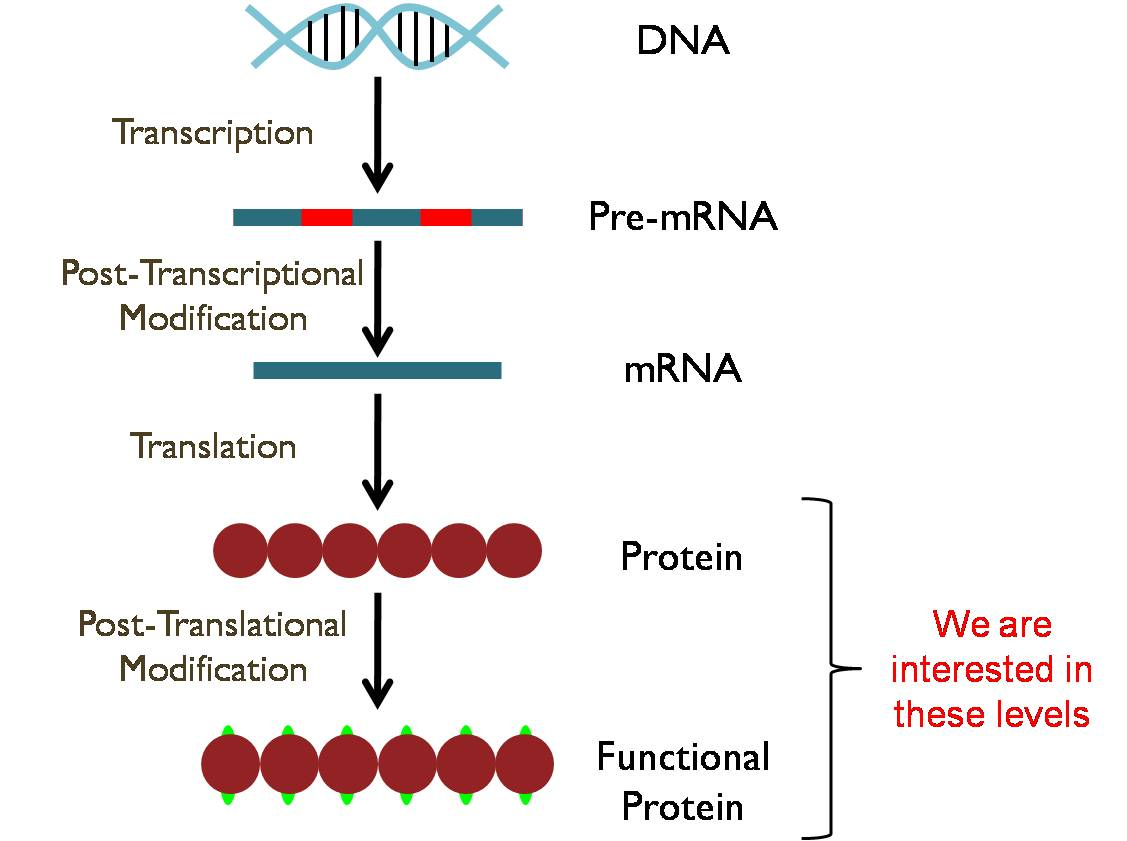
\includegraphics[scale=0.55]{image/processes.jpg}}
\caption{Basic biological processes of producing functional proteins from DNA.}
\label{fig:processes}
\end{figure}

The proteome is the entire complement of proteins expressed by the genome in a cell, or in tissue or bio-fluid of an organism at a given time under specific conditions \citep{Boehm2007}. The function of a protein corresponds to the timing and location of its expression. Proteomic research thus aims to identify and localise many more unknown and known proteins and better understand their functions. 

There are many ways to study proteins. For example, the physical structure of a protein can be studied by X-ray crystallography~\citep{Blow2002}, protein-protein interactions can be studied using the yeast two-hybrid system~\citep{Fields1989}, and the abundance of an individual protein under a defined condition can be studied using isotopic-labelling. The latter is also referred to as \emph{quantitative proteomics}. The use of Multi-dimensional Protein Identification Technology (MudPIT) together with isobaric Tags for Relative and Absolute Quantitation (iTRAQ$^{\rm TM}$) is just one technology used to measure protein abundance.  

\subsection{Multi-dimensional Protein Identification Technology} \label{subsec:MudPIT}
MudPIT is the process of separating a protein complex or peptide mixture using the properties of amino acids, usually into three orthogonal dimensions~\citep{Washburn2001}. Typically, the first separation is by charge, using \emph{strong cation exchange chromatography} (SCX). This is followed by a second separation by hydrophobicity, using \emph{reversed phase liquid chromatography} (RPLC). The third separation is by mass, and is carried out by \emph{mass spectrometry} (MS). This reduces the complexity of the sample and enables high throughput protein analysis. Each MudPIT \emph{run} thus comprises these three steps of separation.

The SCX column contains immobilised negatively charged sulfonic acids that form an ionic interaction with the positively charged peptides. Hence, the charge separation by SCX divides a protein digest (i.e. a mixture of peptides) into many different fractions based on the strength of charge interaction between the peptides and sulfonic acids. Different peptide sequences have different affinities for the SCX resin. This allows for complex peptide mixtures to be fractionated by gradually increasing the concentration of a competing salt solution (for binding to the sulfonic acid groups in a gradient) in a step-wise manner. The salt concentration ranges between 10mM to 500mM. Hence, at each interval of salt concentration, a set of peptides is released into the next MudPIT phase. Each of these charge intervals is termed a \emph{salt step}, and increasing the number of salt steps enables the detection of proteins with low abundance. 

The set of peptides from each charge fraction are then separated by RPLC based on hydrophobicity. This is achieved with a separate column that contains silica beads with chains of 18 carbon atoms attached. The peptides are loaded into the column, which causes hydrophobic interactions with the carbon chains. An organic solvent is then added to the column in concentrations that increase over time, causing the peptides to emerge or \emph{elute}, with the least hydrophobic peptides eluting first. Eluted peptides are then detected using the mass spectrometer.

The mass analysis is performed by MS, whereby each peptide's \emph{mass-to-charge ratio} (m/z) is measured and the measurements are then used to calculate the molecular mass. Peptide separation is described in more detail in \cite{Eidhammer2008}. 

\emph{Tandem mass spectrometry} (MS/MS), which consists of two repeated phases of MS, was used for this study. Peptide fragmentation occurs between the two phases of MS, and identification and quantification of the peptides and proteins is thus based on these peptide fragments. MS/MS enables higher specificity in protein identification and enables more accurate quantification.

MudPIT has some limitations. For example, large variation in signal intensity between different MudPIT runs can make inter-sample comparisons of peptide or protein abundance difficult. This limitation has been resolved by iTRAQ$^{\rm TM}$ labelling, which enables the simultaneous analysis of up to eight distinct protein digests within a single MudPIT run. For this thesis, each MudPIT run is referred to as a \emph{run}. 

\subsection{iTRAQ$^{\rm TM}$ for Protein Quantitation}\label{subsec:iTRAQ}
In its initial format, introduced by \cite{Ross2004}, iTRAQ comprised four isobaric tags, each comprising a reporter group, balance group and peptide reactive group. The reactive group binds the N-terminus at the start of each peptide, and, if the peptide contains lysine residues (i.e. amino acid), then also on the lysine's side chain. The m/z values of the four reporter groups range from 114 to 117, with corresponding balance group values that range from 31 to 28. Each of the four tags thus has an identical total m/z value of 145, making them isobaric. This enables identical peptide species, differentially labelled with the four tags, to be indistinguishable with respect to the intact mass of the peptide when selected for MS/MS~\citep{Ross2004}. For MS/MS, the relative abundances are determined using the reporter ion signals at m/z values of 114, 115, 116 and 117 on the \emph{mass spectrum}. A mass spectrum is a graphical representation of the peptides and peptide fragments based on their m/z values and abundances, and is generated for both phases of MS/MS. The four different labels thus allow the simultaneous analysis of four different samples ~\citep{Ross2004}.
 
\begin{figure}[htb]
\centering{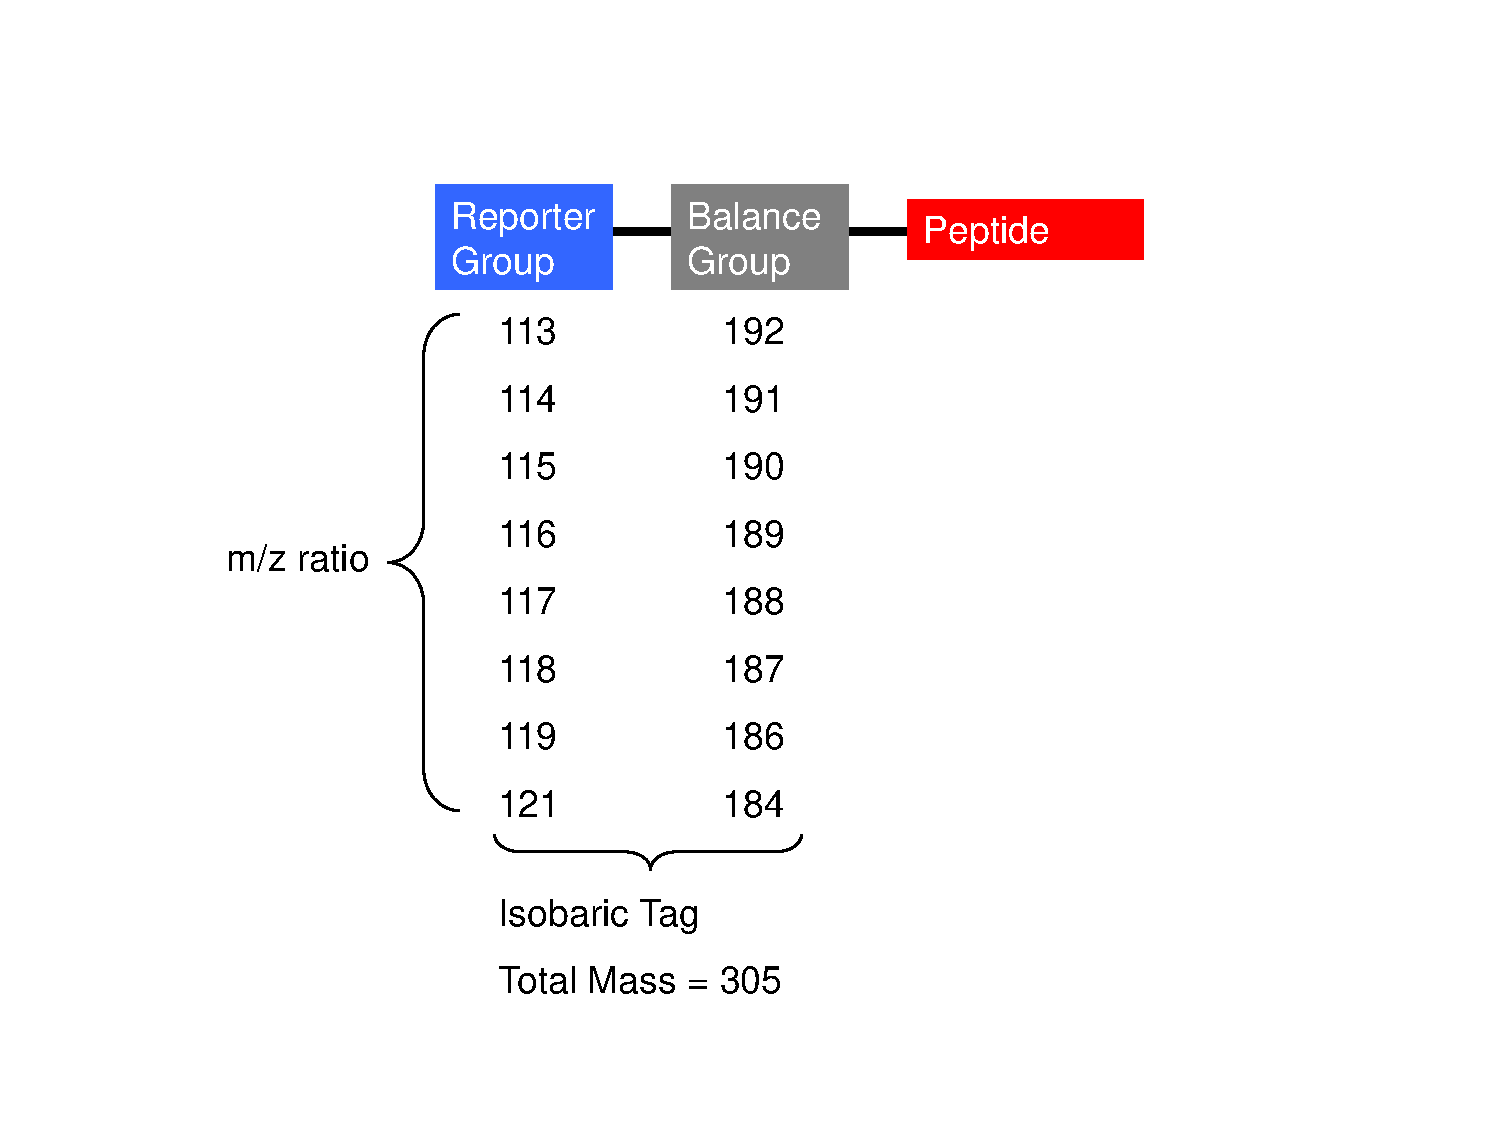
\includegraphics[scale=0.6]{image/iTRAQtags.pdf}}
\caption{Structure of eight-plex-iTRAQ$^{\rm TM}$ tags showing the reporter and balance group masses measured using m/z~\citep{Choe2007}.}
\label{fig:eight-plex}
\end{figure}

\cite{Choe2007} described a new multiplexing strategy, based on the same concept as the four-plex iTRAQ$^{\rm TM}$ system, that allows the simultaneous analysis of up to eight distinct protein samples (see Figure~\ref{fig:eight-plex}). The scheme involves reporter ion signals located at m/z values of 113, 114, 115, 116, 117, 118, 119 and 121. No label is used for an m/z of 120 because it has the same mass as the phenylalanine immonium ion~\citep{Pierce2008}.  For this thesis, each iTRAQ$^{\rm TM}$ tag is referred to as a \emph{tag}. 

\section{Experimental design for proteomic experiments by Oberg}
\label{sec:oberg}
\cite{Oberg2009} have discussed the principles of experimental design for the mass spectrometry-based proteomic experiments, which include the MudPIT-iTRAQ$^{\rm TM}$ experiments. The goal of an experimental design is to allocate individual samples to tags and runs in a way that avoids systematic bias and reduces the error variance of treatment comparison using the ANOVA table. 

\cite{Oberg2009} recognised that each MudPIT run as a block; thus the treatment allocation to runs can be arranged as either a randomised complete block design (RCBD) or a balanced incomplete block design (BIBD). In the RCBD, the number of treatments is the same as the number of tags, while in the BIBD, the number of treatments exceeds the number of tags. Two additional designs were also discussed: the reference design and loop design. The reference design is where each run contains a reference sample for comparison, while the loop design is where the samples are allocated such that they are cycled through the blocks systematically. Upon comparing between the error variances of treatment comparison between the design, \cite{Oberg2009} concluded that the RCBD is most ideal, because it requires fewer runs. Additionally, if a run is lost, this is equivalent to reducing one set of biological replicates. Meanwhile, the resultant design still retains a balanced structure. However, if the loss of runs occurs in the BIBD and loop design, the resultant design may not preserve the balanced structure, i.e.\ the replications of the each treatment becomes not identical. The reference design is most robust under run failure, but may require the largest number of runs for the additional reference sample. Given that the number of tags can be either 4 or 8, then given the high costs of performing the experiment in each MudPIT run, the biologists are likely to utilise all the tags. The RCBD thus may not be possible in all circumstances, because the biologists are unlikely to continuously compare only 4 to 8 conditions. 

\cite{Oberg2012} again recognised that allocation of treatments to runs and tags is a randomised block design, where the MudPIT run is the block factor. Moreover, \cite{Oberg2012} suggested that multiple MudPIT runs are required to avoid the confounding of tag effects with treatment effects.

Furthermore, the \cite{Oberg2009} and \cite{Oberg2012} only consider the allocation of treatments to runs and tags. The allocation of any other block factors, e.g. animals or plants, is equally important, because it can also affect the error variance of treatment comparison. Therefore, such experiments must be treated as two-phase experiments.  


\section{Overview}
\label{sec:overview}
The main aim of this thesis is to develop a general construction methodology for two-phase experiments when the Phase~2 experiment involves either a four- or eight-plex iTRAQ$^{\rm TM}$ proteomics experiment. Such a methodology can be divided into three main parts, as follows. 

As mentioned by \cite{Brien2011}, the ANOVA tables with the EMS for two-phase experiments are valuable for comparing the properties of different experimental designs. Chapter 2 first describes a decomposition method for single- and two-phase experiments used to construct the ANOVA table with the EMS. Since no existing tool can automatically generate such tables, an \textsf{R} package called \textbf{infoDecompuTE} is developed that allows the researchers to generate the ANOVA table with EMS by entering any single- or two-phase experimental design. 

For a given set of design parameters, there are often many ways to allocate the samples collected from the Phase~1 experiment to the blocks of the Phase~2 experiment. The computational method used to find the optimal designs for different classes of design, such as block, row-column and $\alpha_n$ designs, has previously been discussed \citep{whitaker1990, Williams1996, John2002}. However, such a method has not yet been developed for optimizing the design of the two-phase experiment. Chapters 3 and 4 thus developed the computer based methods of generating two-phase optimal designs by optimising the objective function using the \emph{simulated annealing algorithm} (SA). The optimality criterion is defined in the \emph{objective function}, which is a mathematical expression generating a numeric value. SA is a well-known heuristic method for finding the input, in this instance the candidate design, that maximizes or minimizes the value generated from this objective function \citep{Kirkpatrick1983}. Additionally, Chapters 3 and 4 further improve the SA in terms of both the speed and efficiency of finding the optimal design. Using the MudPIT-iTRAQ$^{\rm TM}$ experiment as the primary example, the objective function and SA are defined and developed to design an experiment where the Phase~1 experiment involves a completely randomised design (Chapter 3) and a randomised block design (Chapter 4). Furthermore, \cite{Brien2009, Brien2010} only considered balanced designs, which contain a set of identical efficiency factors for every DF associated with a given block or treatment factor. Chapters 3 and 4 present some optimal designs that are not balanced.


Chapter 5 compares several properties of the optimal designs found in Chapters 3 and 4. Firstly, Chapter 5 shows how to estimate the variance components using the restricted maximum likelihood (REML) based on the model that describes the experimental structure of the design. As mentioned in Section~\ref{sec:Jarrett2008}, the information of the experimental units from the Phase~1 experiment can be recovered from the Between Blocks analysis of the Phase~2 experiment, which allows the estimation of the EDF. The EDF, using the variance component estimates, can be computed from the first two moments of the chi-square distribution \citep{Satterthwaite1946}. The comparison of some optimal designs found in Chapters 3 and 4 using the EDF can help clarify the properties of different candidate designs. 

Chapter 6 summarises and concludes the entire thesis. Furthermore, it also presents future directions in the design and analysis of the two-phase experiment, particularly, for the quantitative high-throughput biotechnologies experiment with multiplexing technology which is currently useful and will remain so for the next decade.   

\bibliographystyle{apalike}
\bibliography{ref}

\end{document}
